\section{Implementierung der einheitlichen Speicherlösung}\label{implementierung_ssot}

Die nachfolgend beschriebene Implementierung ist als Proof of Concept im Open-Source-Projekt \code{ArkAutomate}\footnote{\url{https://github.com/bptlab/ark_automate} (Abgerufen am 22. Juni 2021)}  umgesetzt. Die Entwicklung erfolgte im Rahmen des der Abschlussarbeit zugrunde liegenden Projektes. Das Projektteam implementierte die in dieser Arbeit beschriebene einheitliche Datenspeicherlösung sowie die Modellierungsfunktion als ein Kernfeature der quelloffenen RPA-Plattform. Die SSoT ist in diesem Projekt als verschachteltes JavaScript Object implementiert. 

Betrachten wir nun das beidseitige Parsing zwischen der visuellen Repräsentation und der SSoT. Wie im vorangegangenen Kapitel beschrieben, werden zwischen jedem Interface und der SSoT zwei Parser benötigt. Ein Parser übersetzt das Modell in die SSoT und ein weiterer Parser erstellt aus der SSoT die visuelle Repräsentation.

Die Implementierung der Parser hängt stark von dem verwendeten Modellierungsmodul ab. Das im Proof of Concept verwendete npm-Paket \code{bpmn-js}\footnote{\url{https://www.npmjs.com/package/bpmn-js} (Abgerufen am 22. Juni 2021} zeichnete sich durch seine umfangreichen Funktionen und Anpassungsmöglichkeiten des Modelers aus. Zur Modellierung von Flowcharts bietet sich eine Erweiterung des \code{react-flow-diagram} Paketes\footnote{\url{https://www.npmjs.com/package/react-flow-diagram} (Abgerufen am 22. Juni 2021)} an. Es lässt sich um die unterstützten Sinnbilder erweitern. Einen Modeler-Package zur Erstellung von Ereignisgesteuerten Prozessketten konnte nicht gefunden werden. Dies kann an der geringen Verbreitung der Notation außerhalb des deutschsprachigen Raumes liegen.

Nachfolgend werden die grundlegenden Konzepte der Parser an den im Proof of Concept verwendeten Notationen BPMN und dem finalen Ausführungscode beschrieben.

\subsection{Übersetzung der SSoT in eine visuelle Repräsentation}

Betrachten wir zuerst den Parser, der den RobotFramework Code erzeugt. Zu Beginn dieses Codes müssen die verwendeten RpaFramework Librarys aufgeführt werden (Abbildung \ref{fig:ScrRobotFr}). Hierfür genügt eine Iteration über das \code{ElementArray}, bei der alle verwendeten Applikationen gespeichert werden. Der Graph lässt sich mit einer rekursiven Betrachtung des \code{ElementArray}s rekonstruieren, wodurch der RobotFramework Code zeilenweise wächst. 

Komplizierter hingegen ist die Erstellung von Modellen aus der SSoT. Hierbei sind die verwendeten XMLs oft sehr komplex und erfordern eine Vielzahl an Parametern wie Positionen der Elemente und Verbindungen. Für das Paket \code{bpmn-js} existiert jedoch ein Command Line Interface (CLI)\footnote{\url{https://www.npmjs.com/package/bpmn-js-cli} (Abgerufen am 22. Juni 2021)}, das die Ausrichtung der BPMN-Komponenten übernimmt. So genügt es, dem BPMN-Diagramm die Elemente in der sortierten Reihenfolge mittels \code{cli.append(element)} hinzuzufügen. Das anzuzeigende XML mit allen Positionswerten wird durch das Interface erstellt.  

\subsection{Übersetzung einer visuellen Repräsentation in die SSoT}

Zur einfacheren Speicherung der Informationen eines Roboters wird in der Implementierung der eigentliche Graph getrennt von den Eigenschaften jedes Knotens gespeichert. Die Informationen zu \code{rpaApplication} und \code{rpaTask} werden zusammen mit einer Referenz auf das betreffende \code{INSTRUCTION}-Element in der \code{localAttributeStorage} abgelegt. In diesem einen Objekt der Session Storage werden somit direkt alle Änderungen an der \mbox{RPA Task / Application-Kombination} vermerkt. Das \code{localParameterStorage}-Objekt speichert zu jedem \code{INSTRUCTION}-Element ein Array aller Parameter mit den in Abbildung \ref{fig:aufbauSSOT} vorgestellten Feldern. Die Seitenleiste (\code{ModelerSidebar}) bietet die Möglichkeit, alle Parameter eines Elements zu verändern. Die Änderungen werden direkt in den betreffenden Objekten der Session Storage geändert. Die \code{ModelerSidebar} ist modular aufgebaut und kann daher weiteren in Modellierungsinterfaces wiederverwendet werden.

Betrachten wir nun das Parsing - die eigentliche Erstellung der SSoT. Hierbei lassen sich für alle Parser dieser Richtung einige Gemeinsamkeiten festhalten. Jeder Parser erstellt zuerst den SSoT-Header mit den beschriebenen drei Feldern. Im Anschluss muss das \code{ElementArray} erstellt werden, sodass dann beide Teile zur SSoT zusammengefügt und gespeichert werden können. 

Sofern die Daten in einer nicht strukturierten Form vorliegen, müssen sie vorab aufbereitet werden. Dieser Schritt geschieht beim RobotFramework Code durch zeilenweises Einlesen. Die Daten des \code{bpmn-js} liegen im XML-Format vor und müssen daher ebenso vorab bearbeitet werden. Das XML lässt sich in der JavaScript Anwendung schwer verarbeiten, weshalb es in der Projektarbeit mit dem \code{xmljs2}-Paket\footnote{\url{https://www.npmjs.com/package/xmljs2} (Abgerufen am 22. Juni 2021)} in ein JavaScript Objekt gewandelt wurde. Auf dieser Grundlage können die Elemente durch eine einfache Iteration über die strukturierten Daten erstellt werden. Der BPMN-Parser muss das \code{bpmn-js}-XML um die Informationen der ausgelagerten Objekte aus der Session Storage anreichern.  

\subsection{Evaluation der Lösung}
\label{evaluation_ssot}

Die vorgestellte Lösung, die in ersten Teilen im Proof of Concept implementiert wurde, ermöglicht das Bearbeiten der Roboter in verschiedenen Modellierungssprachen. Die Parser, die aus der SSoT die visuelle Repräsentation des Roboters erstellen, ließen sich leicht implementieren. Das lag vor allem an dem durch Camunda bereitgestellten Interface sowie dem \code{bpmn-js} Modeler. Sofern diese Tools für eine Modellierungssprache - wie beispielsweise die EPKs - nicht zur Verfügung stehen, erhöht sich der Arbeitsaufwand zur Anbindung weiterer Interfaces erheblich. Aufwändig ist vor allem das korrekte Ausrichten der Elemente des Modells, was im Beispiel des BPMN-Editors das CLI übernahm.

Die Parser, die beim Speichern den Roboter in die SSoT übersetzen, implementieren sich vergleichsweise komplizierter. Um Fehler bei der Erstellung der SSoT zu vermeiden, ist eine komplexe Fehlerbehandlung notwendig, die unsaubere Eingaben des Codes abfängt. Gleiches gilt für den Parser, der das BPMN-Diagramm in die SSoT übersetzt. Sobald ein Fehler beim Übersetzen festgestellt wird, bricht der Parser ab und es wird keine SSoT an den Server gesendet. Bei beiden Parsern wird ein besonderer Fokus auf aussagekräftige Fehlermeldungen gelegt, die den Nutzern bei der Bedienung helfen. So wird der Entwickelnde unter anderem gewarnt, wenn das BPMN-Modell zwei Start-Ereignisse besitzt (Abbildung \ref{fig:errorBPMN}) oder wenn ein Schreibfehler im Code-Editor erkannt wird (Abbildung \ref{fig:errorROBOT}).

\begin{figure}[!htb]
    \centering
    \begin{minipage}{.5\textwidth}
        \centering
        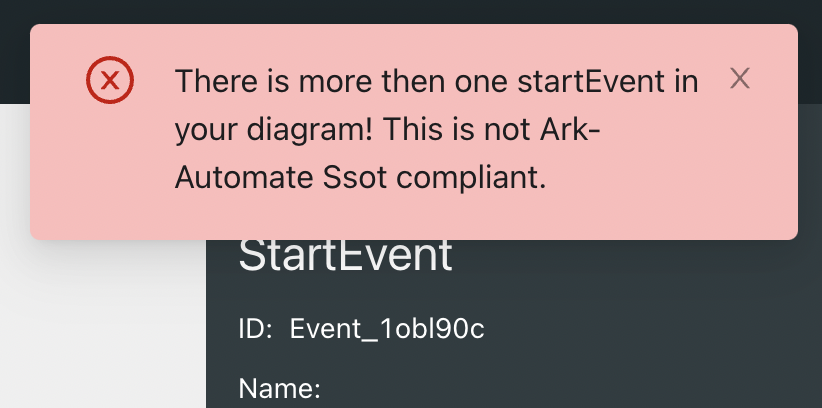
\includegraphics[width=0.95\textwidth, height=0.17\textheight]{Bachelorarbeit/images/ScreenshotErrorBPMN3.png}
        \caption{Fehlermeldung \\ BPMN-Editor}
        \label{fig:errorBPMN}
    \end{minipage}%
    \begin{minipage}{0.5\textwidth}
        \centering
        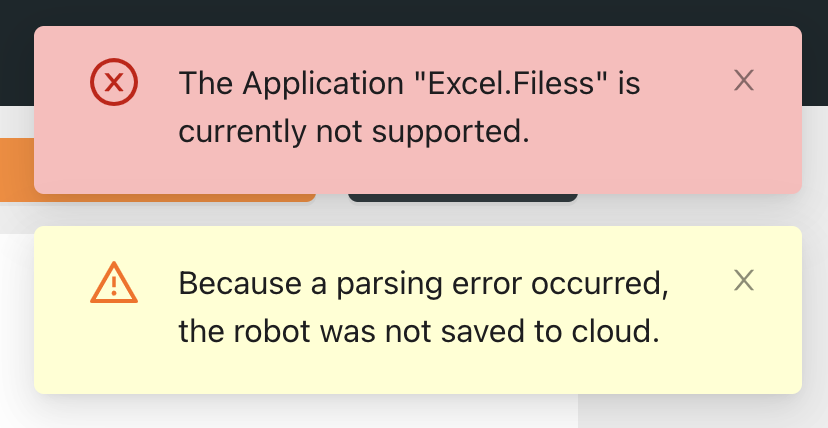
\includegraphics[width=0.95\textwidth, height=0.17\textheight]{Bachelorarbeit/images/ScreenshotErrorROBOT.png}
        \caption{Fehlermeldung \\ Code-Editor}
        \label{fig:errorROBOT}
    \end{minipage}
\end{figure}

Das Proof of Concept unterstützt aktuell die Element-Typen \code{MARKER} und \code{INSTRUCTION}. Um weitere Typen zu unterstützen, ist eine Umstellung des \mbox{RobotFramework} Codes auf die Keywords-Syntax notwendig. Hierfür müssen die zwei betreffenden Parser angepasst werden. Die Keywords-Syntax ermöglicht das Zusammenfassen von Programmteilen ähnlich der Definition von Funktionen in der objektorientierten Programmierung. Diese Funktionen werden als Keywords bezeichnet und im Hauptprogramm semantisch aneinandergereiht (Abbildung \ref{fig:ScrRobotFrKeywords}). Sobald diese Umstellung erfolgt, lassen sich auch die beschriebenen Konzepte der Schleife und der Verzweigung implementieren. Mit der Weitentwicklung der Plattform ließe es sich zudem implementieren, einzelne Programmbausteine mehrfach zu verwenden.

Aus meiner persönlichen Erfahrung heraus ist die Bedienung des RobotFramework Editors sehr umständlich. Prinzipiell lassen sich im Code-Editor Automatisierungen mit weniger Klicks implementieren als im BPMN-Editor, jedoch fehlen vor allem eine Auto-Vervollständigung sowie eine Schnellvorschau beim Schreiben des Codes. Aktuell existiert keine Möglichkeit, die Aktivitäten einer Library sowie  die benötigten Parameter angezeigt zu bekommen. Daher ist das Programmieren momentan nur für Experten, die alle zu verwendenden Befehle kennen, möglich. In Zukunft kann die Weiterentwicklung des Robot Framework Language Servers\footnote{\url{https://marketplace.visualstudio.com/items?itemName=robocorp.robotframework-lsp} \\ (Aufgerufen am 24.07.2021)} eingebunden werden, die eine Code-Vervollständigung sowie Syntax-Validierung unterstützt.

Aus meiner Sicht bietet es sich an, für erfahrenere Entwickler, die keine Erfahrung in der Modellierung haben, ein Low-Code-Interface wie Google Blockly\footnote{\url{https://developers.google.com/blockly} (Abgerufen am 12.07.2021)} bereitzustellen. Google Blockly ermöglicht die Programmierung in einem grafischen Code-Editor durch die Aneinanderreihung von Funktionsblöcken. Blockly ist unter anderem die dem grafischen Code-Editor zugrunde liegende Library des  MIT AppInventors. 

